\documentclass[conference]{IEEEtran}
\usepackage[utf8]{inputenc}
\usepackage[spanish]{babel}
\usepackage{multirow}
\usepackage{amsmath}
\ifCLASSINFOpdf
\usepackage[pdftex]{graphicx}

\else
\fi
\hyphenation{op-tical net-works semi-conduc-tor}

\begin{document}
\title{Comparación de las técnicas de modulación SPWM Unipolar y SPWM Bipolar en inversores monofásicos con cargas RL}
\author{
		\begin{tabular}{c}
			\textbf{Hernando, Diego Joaquín - djhernando96@gmail.com} \\ 
			Estudiante de Ingeniería Electrónica - Universidad Tecnológica Nacional - Facultad Regional Córdoba
		\end{tabular}
		}
\maketitle

\begin{abstract}
Se describirá el funcionamiento de inversores monofásicos con técnicas de modulación SPWM Unipolar y Bipolar, comparando las señales de mando de los dispositivos de conmutación, tensiones y corrientes de salida del inversor. Por último se hará un análisis de contenido espectral en la señal de salida para distintos valores de índice de modulación en amplitud e índice de modulación en frecuencia. El estudio se llevará a cabo por medio de simulaciones en el software OrCad PSpice.\\


\textit{Abstract}---Describe the operation of inverters with SPWM Unipolar and Bipolar modulation, comparing the control signals of switching devices, voltage and current output of the inverter. Finally, an analysis of spectral content in the output signal for different values amplitude modulation index and index modulation frequency. The simulation work will be held in Orcad PSpice. 
\end{abstract} 

\IEEEpeerreviewmaketitle

\section{Introducción}
Los inversores son convertidores que trasfieren potencia desde una fuente de continua a una carga de alterna. Su función es cambiar la tensión de entrada de CC, a una tensión de salida simétrica de CA, con magnitud, fase y frecuencia deseadas.

En la mayoría de los casos, es necesario controlar la tensión de salida de los inversores, ya sea para regular variaciones de la tensión de alimentación o para regular la tensión en la carga. Esto se logra modulando el ancho de pulso que comanda los transistores de potencia. Algunos métodos son: control por decalado, por múltiples pulsos, modulación senoidal del ancho de pulso SPWM, modulación del vector espacial, entre otros. Todos estos métodos tiene el mismo fin, sin embargo algunos mejoran ciertas características que otros no, como por ejemplo el manejo de la tensión de salida y el control de armónicos. El uso de estos métodos dependerá de la necesidad de la aplicación.

Los inversores se utilizan en la industria tanto en aplicaciones monofásicas como trifásicas. Algunos usos son: control de giro y velocidad de un motor de CA, UPS, conversión de energía CC/CA en fuentes de energía renovables, entre otros. 	

\section{Inversor Monofásico}
El circuito utilizado para la simulaciones es el que se observa en la Fig. \ref{fig:circuito}. Los transistores de potencia son representados por llaves controladas por tensión. 
\begin{figure}[t]
	\centering
	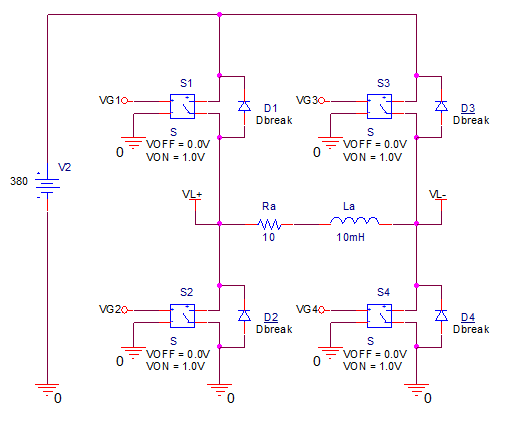
\includegraphics[width=8cm]{imagenes/circuito}
	\caption{Circuito esquematico de inversor monofásico}
	\label{fig:circuito}
\end{figure}

\section{Modulación senoidal por ancho de pulso SPWM}
Esta técnica consiste en generar las tensiones de comando de compuerta de los transistores de potencia a partir de la comparación de una señal portadora o triangular y una señal de referencia, moduladora o senoidal. El resultado son pulsos cuadrados de distintos anchos que modulan la conmutación de los transistores.

Es posible definir el índice de modulación en amplitud y el índice de modulación en frecuencia, de acuerdo a las señales antes mencionadas, tal como se observa en las ecuaciones \ref{ecu:ma} y \ref{ecu:mf}.

\begin{equation}
	m_a = \frac{V_{max - referencia}}{V_{max - portadora}}
	\label{ecu:ma}
\end{equation}
\begin{equation}
	m_f = \frac{f_{portadora}}{f_{referencia}}
	\label{ecu:mf}
\end{equation}

Esta técnica logra disminuir la distorsión armónica total ($THD$) de forma considerable.

\section{SPWM Bipolar}
\subsection{Señales de control}
Esta técnica consiste en conmutar simultaneamente los transistores de una diagonal del inversor. Es decir, las llaves S1 y S4 se activan cuando $V_{referencia} > V_{portadora}$, y las llaves S2 y S3 en caso contrario. Se observa que sólo es necesario dos señales de control, las cuales se observan en la Fig. \ref{fig:controlbi}.

\begin{figure}[t]
	\centering
	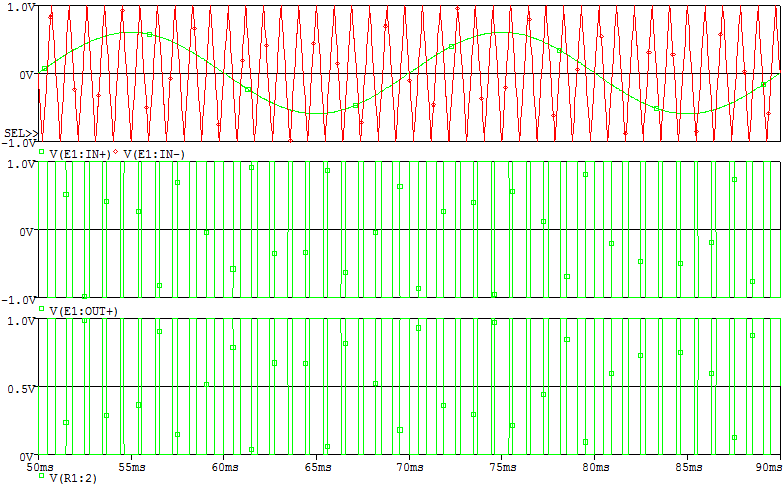
\includegraphics[width=8cm]{imagenes/bipolar/Control}
	\caption{Comparación de señal portadora y de referencia. Generación de señales de conmutación para $m_a = 0.6$ y $m_f = 21$.}
	\label{fig:controlbi}
\end{figure}
\subsection{Señal en la carga}
La tensión en la carga es una señal PWM Bipolar porque es alternada entre positivo y negativo en cada conmutación de las llaves. La forma de onda de corriente presenta quiebres debido a las propiedades del inductor, se puede ver que los quiebres coinciden con la conmutación de las llaves. La frecuencia de la señal de salida depende de la frecuencia de la señal de referencia. Todo esto se observa en la Fig. \ref{fig:cargabi}.
\begin{figure}[b]
	\centering
	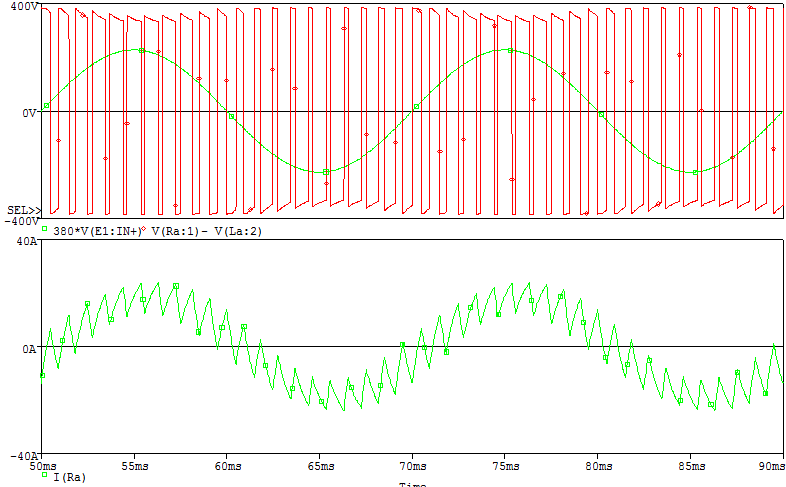
\includegraphics[width=8cm]{imagenes/bipolar/Carga}
	\caption{Tensión y corriente de carga para $m_a = 0.6$ y $m_f = 21$.}
	\label{fig:cargabi}
\end{figure}
\subsection{Efectos del $m_a$ en la señal de salida}
Es posible compensar las variaciones en la alimentación de CC que excita al inversor modificando $m_a$, teniendo en cuenta que para $m_a \leq 1$ la amplitud de la primer armónica será proporcional a $m_a$, es decir, $\hat{V}_{1} = m_a \cdot V_{in}$.
En las Fig. \ref{fig:ma0bi} y \ref{fig:ma1bi} se observa la amplitud de la fundamental
($50$ $Hz$) para distintos $m_a$, manteniendo constante $m_f = 21$.
\begin{figure}[t]
	\centering
	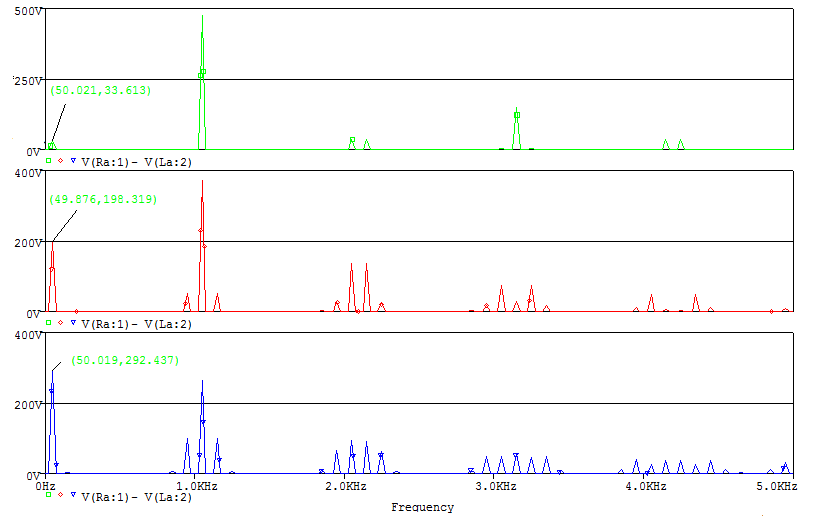
\includegraphics[width=8cm]{imagenes/bipolar/ma0}
	\caption{Componentes armónicos para $m_a = 0.1, 0.6$ y $0.9$.}
	\label{fig:ma0bi}
\end{figure}
\begin{figure}[b]
	\centering
	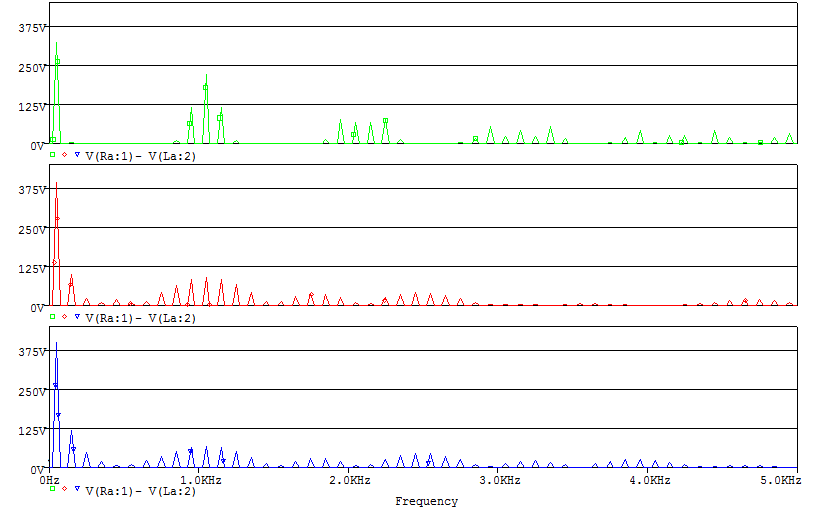
\includegraphics[width=8cm]{imagenes/bipolar/ma1}
	\caption{Componentes armónicos para $m_a = 1, 2$ y $3$.}
	\label{fig:ma1bi}
\end{figure}
Por un lado se observa que la tensión de la fundamental crece linealmente proporcional a $m_a$ cuando este es igual o menor que 1. Para $m_a$ mayor que uno el crecimiento deja de ser proporcional y se presenta el caso de sobremodulación, que lleva a la saturación del sistema de control y a la obtención de una señal de salida cuadrada. Por otro lado, se observa que a medida que aumenta $m_a$ aparecen componentes armónicos cada vez mas cercanos de la fundamental complicando el filtrado de la señal de salida. Estos resultados se observan claramente en la siguiente tabla y en la Fig. \ref{fig:thdbi}.

\begin{center}
\begin{tabular}{|c|c|c|}
		\hline
	$m_a$& $V_1$ $[V]$ & $THD$ [\%] \\ 
	\hline 
	0.1 & 33.01 & 2596 \\ 
	0.2	& 67.64 & 729\\ 
	0.3	& 100.48 & 495 \\ 
	0.4 & 132.01 & 393 \\ 
	0.5 & 165.63 & 325 \\ 
	0.6 & 197.34 & 241 \\ 
	0.7 & 228.72 & 182 \\ 
	0.8 & 262.76 & 163 \\ 
	0.9 & 291.29 & 122 \\ 
	1 & 312.56 & 115 \\ 
	2 & 393.72 & 66.6 \\ 
	3 & 400.17 & 57.1 \\ 
	\hline 
\end{tabular} 
\end{center} 

\begin{figure}[t]
	\centering
	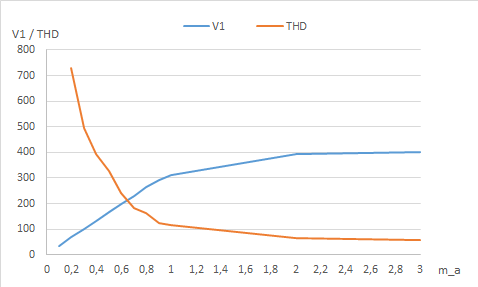
\includegraphics[width=8cm]{imagenes/bipolar/thd}
	\caption{Tensión de la fundamental y distorsión armónica total en función de $m_a$.}
	\label{fig:thdbi}
\end{figure}

\subsection{Efecto del $m_f$ en la señal de salida}
La Fig. \ref{fig:mfbi} muestra que a mayor $m_f$, el contenido armónico de desplaza mucho más arriba en
frecuencia que la fundamental, lo que facilita el filtrado de la señal para obtener la fundamental pura. Además, se observa que para para un $m_f$ no entero aparecen subarmónicos que dificultan el filtrado de la señal de salida, razón por la cual se utilizan valores enteros.

\begin{figure}[b]
	\centering
	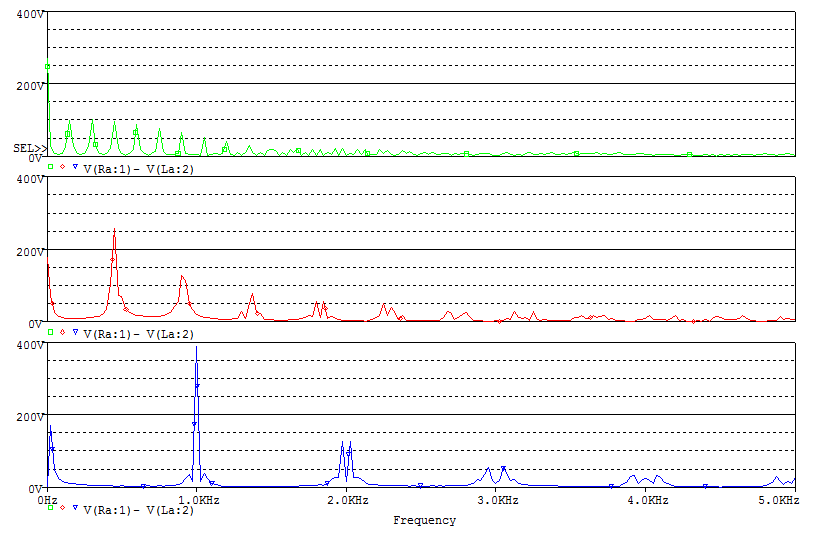
\includegraphics[width=8cm]{imagenes/bipolar/mf}
	\caption{Contenido espectral de la tensión de salida para $m_f = 3, 9.12$ y $20$ con $m_a = 0.6$.}
	\label{fig:mfbi}
\end{figure}

\section{SPWM Unipolar}
\subsection{Señales de control}
A diferencia del caso Bipolar, las ramas del inversor se controlan de forma independiente. Es decir, S1 se activa cuando $V_{referencia} > V_{portadora}$. S2 es el caso contrario de S1. S3 se activa cuando $- V_{referencia} > V_{portadora}$ y S4 en caso contrario. Se tienen cuatro señales de control, las cuales se observan en la Fig. \ref{fig:controluni}.
\begin{figure}[t]
	\centering
	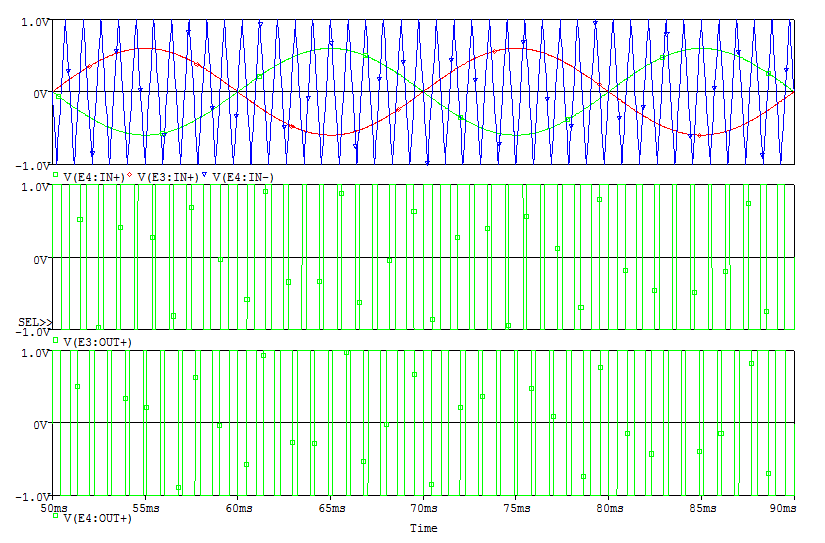
\includegraphics[width=8cm]{imagenes/unipolar/control}
	\caption{Comparación de señal portadora y de referencia. Generación de señales de conmutación para $m_a = 0.6$ y $m_f = 21$.}
	\label{fig:controluni}
\end{figure}
\subsection{Señal en la carga}
La tensión en la carga es una señal PWM Unipolar porque es alternada entre cero y un valor positivo o negativo en cada conmutación de las llaves. La corriente que circula por la carga presenta quiebres en los puntos donde la señal de control conmuta, pero estos quiebres son menos pronunciados que en los Bipolares debido a que los cambios de polarización en la carga son menores en relación al método Bipolar. Nuevamente, la frecuencia de la señal de salida depende de la frecuencia de la señal de referencia. Esto se observa en la Fig. \ref{fig:cargauni}.

\begin{figure}[b]
	\centering
	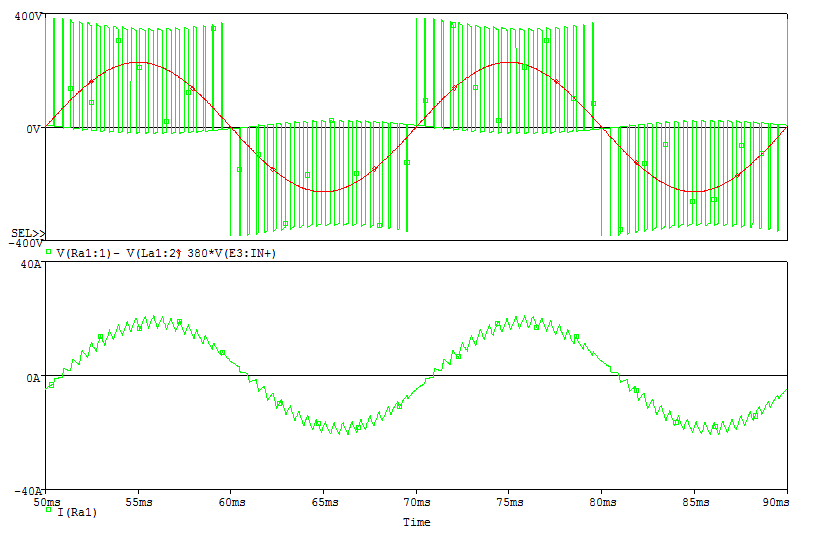
\includegraphics[width=8cm]{imagenes/unipolar/carga}
	\caption{Tensión y corriente de carga para $m_a = 0.6$ y $m_f = 21$.}
	\label{fig:cargauni}
\end{figure}
\subsection{Efectos del $m_a$ en la señal de salida}
Las Fig. \ref{fig:ma0uni} y \ref{fig:ma1uni} muestran la forma en que varia la tensión de la fundamental conforme aumenta $m_a$. La siguiente tabla muestra en detalle la variación de la tensión fundamental y de la distorsión armónica total. La Fig. \ref{fig:thduni} muestra esta variación en función del $m_a$.
\begin{figure}[t]
	\centering
	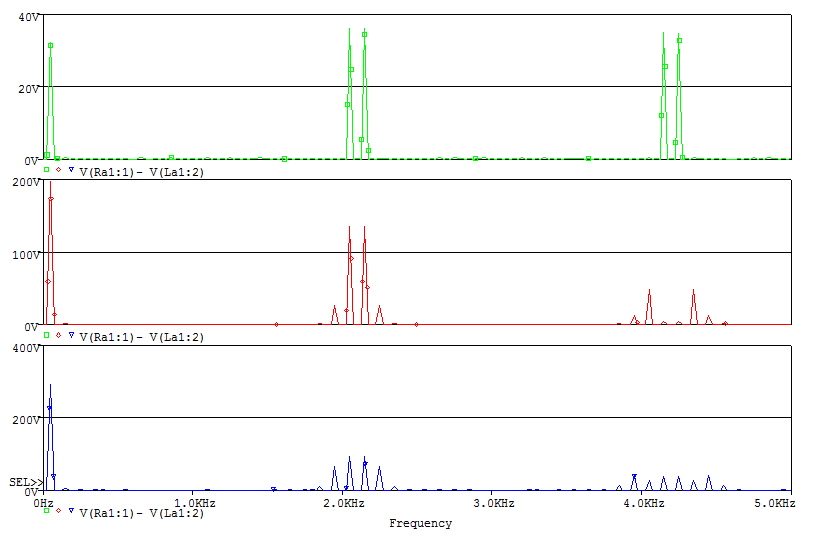
\includegraphics[width=8cm]{imagenes/unipolar/ma0}
	\caption{Componentes armónicos para $m_a = 0.1, 0.6$ y $0.9$.}
	\label{fig:ma0uni}
\end{figure}
\begin{figure}[b]
	\centering
	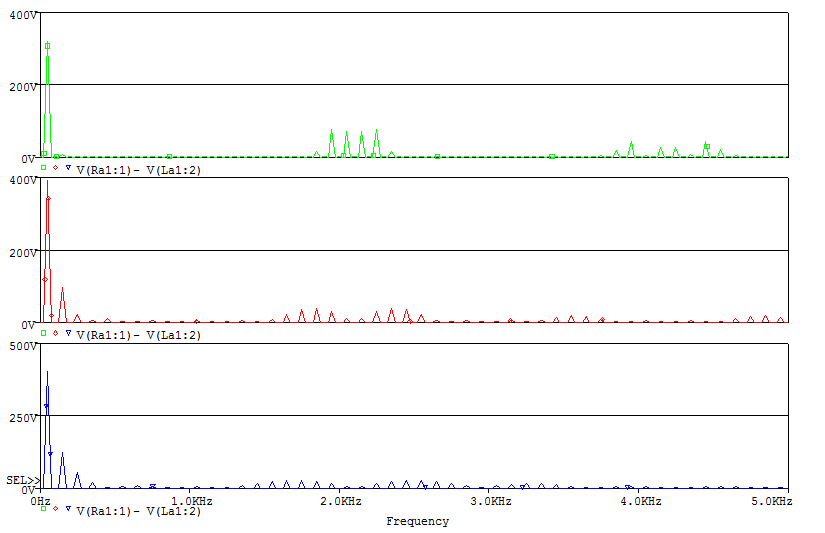
\includegraphics[width=8cm]{imagenes/unipolar/ma1}
	\caption{Componentes armónicos para $m_a = 1, 2$ y $3$.}
	\label{fig:ma1uni}
\end{figure}
\begin{center}
	\begin{tabular}{|c|c|c|}
		\hline
		$m_a$& $V_1$ $[V]$ & $THD$ [\%] \\ 
		\hline 
		0.1 & 33.01 & 376 \\ 
		0.2	& 66.03 & 249\\ 
		0.3	& 100.48 & 195 \\ 
		0.4 & 133.49 & 159 \\ 
		0.5 & 165.72 & 134 \\ 
		0.6 & 198.06 & 112 \\ 
		0.7 & 229.66 & 99 \\ 
		0.8 & 261.24 & 86.6 \\ 
		0.9 & 292.82 & 73.7 \\ 
		1 & 322.96 & 56.7 \\ 
		2 & 387.12 & 38.7 \\ 
		3 & 400.17 & 40.2 \\ 
		\hline 
	\end{tabular} 
\end{center} 

\begin{figure}[t]
	\centering
	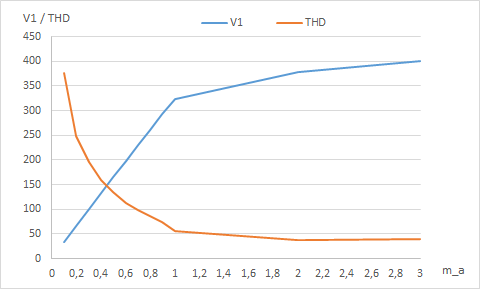
\includegraphics[width=8cm]{imagenes/unipolar/thd}
	\caption{Tensión de la fundamental y distorsión armónica total en función de $m_a$.}
	\label{fig:thduni}
\end{figure}

Se observa que el método unipolar presenta una mejora en la distorsión armónica con respecto al método anterior, manteniendo a la salida aproximadamente el mismo valor de tensión. 

La variación de la tensión fundamental se comporta de la misma manera que en el método Bipolar, mientras $m_a$ es menor que 1 tiene un crecimiento lineal y al superar la unidad el crecimiento es no lineal apareciendo componentes armónicas próximas a la fundamental.

\subsection{Efecto del $m_f$ en la señal de salida}
El método unipolar también facilita el filtrado de la señal desplazando el ruido a altas frecuencias alejandolo de la fundamental, y elimina el contenido armónico que podría aparecer entre la fundamental y los productos de intermodulación. En la Fig. \ref{fig:mfuni} se aprecia lo antes mencionado y se observan que se cumplen las condiciones del $m_f$ al igual que en el Bipolar.

\begin{figure}[b]
	\centering
	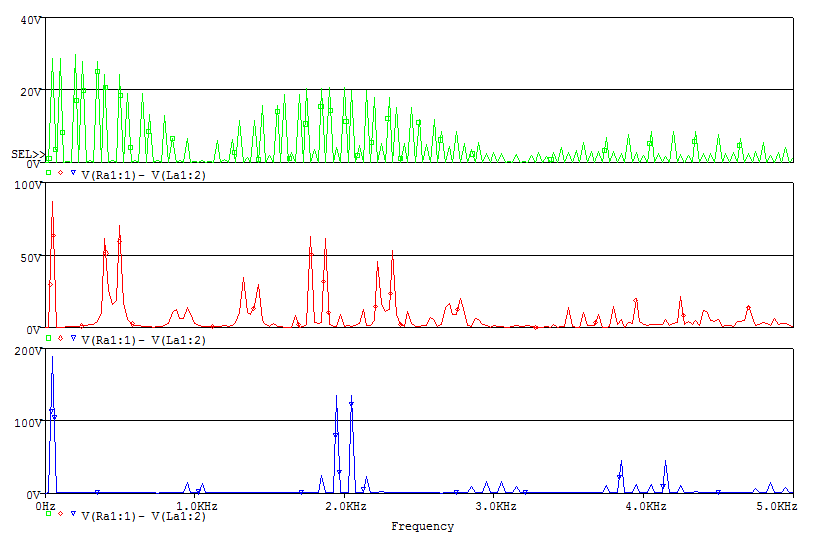
\includegraphics[width=8cm]{imagenes/unipolar/mf}
	\caption{Contenido espectral de la tensión de salida para $m_f = 3$, $9.12$ y $20$ con $m_a = 0.6$.}
	\label{fig:mfuni}
\end{figure}


\section{Conclusiones}
Se observa que tanto los inversores con técnica SPWM Unipolar como SPWM Bipolar tienen como característica la disminución del contenido armónico de la señal de salida, lo cual facilita el filtrado de la misma. La THD disminuye conforme aumenta $m_a$ hasta alcanzar la unidad, momento en el cual la THD vuelve a aumentar debido a que el controlador se satura y se obtiene a la salida del inversor una señal cuadrada. Entre ellos, es el método Unipolar el que presenta la menor distorsión de salida.

Ambos métodos permiten la variación de la señal de salida para compensar las variaciones en la señal de entrada. Estas variaciones de tensión afectan por igual al inversor en los dos métodos de control, haciendo que la tensión de salida sea proporcional a $m_a$ cuando este es menor a la unidad, y presentando, el inversor, una pequeña ganancia cuando trabaja en sobremodulación, pero con algunas consecuencias como es la aparición de componentes armónicas cerca de la señal fundamental ya que la dependencia de la tensión respecto de $m_a$ deja de ser lineal.

En ambos casos se observa que la frecuencia de la señal de salida corresponde a la frecuencia de la señal de referencia. Modificando esta podemos modificar la frecuencia de la señal de alterna resultante. Además es posible modificar la amplitud de la señal de salida modificando $m_a$.

\begin{thebibliography}{1}
	\bibitem{IEEEhowto:kopka}
	Rajashekara, K., Bhat, A.K.S., Bose, B.K. ''Power Electronics'' Ed. Richard C. Dorf, Boca Raton: CRC Press LLC, 2000.
	\bibitem{IEEEhowto:kopka}
	Rashid, Muhammad H., ''Electrónica de potencia'', Pearson Educación, Tercera edición, México, 2004.
	\bibitem{IEEEhowto:kopka}
	Oros, Ramón. ''Electrónica de Potencia''
\end{thebibliography}

\end{document}


